\chapter{Desenvolvimento}
\label{cap:desenvolvimento}

\section{Hello World}

A primeira funcionalidade que foi implementada no projeto foi utilizar-se da biblioteca OpenGL e seguir os passos iniciais para ser possivel desenhar um triangulo na tela. 

Para isso foi implementada uma funcionalidade basica de criação de janela, utilizando-se do SDL2 para que isso fosse multiplataforma e funcionasse com o compilador do Emscripten.

Em seguida foram criadas classes básicas para a criação de shaders, código necessário para que os vertices e pixels da tela sejam coloridos. Após a capacidade de criação de shaders, os pontos de um triangulo foram colocados no loop principal do programa, e utilizando das funções do OpenGL, foi possível renderizar um triangulo conforme a figura \ref{des:glhello}.

\begin{figure}[]
  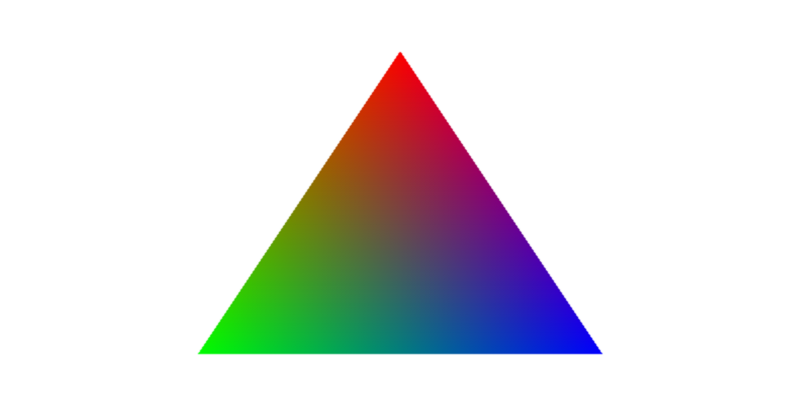
\includegraphics[width=\linewidth]{Cap-Desenvolvimento/glhello.png}
  \caption{Hello World do OpenGL}
  \label{des:glhello}
\end{figure}

\section{Criação de modelos}

A partir do momento que era possivel renderizar um triangulo, a renderização de uma lista de triangulos tornou-se trivial. Assim, o proximo passo do desenvolvimento foi fazer uma função que renderizasse uma lista de vértices quaisquer de um modelo para que fosse possivel renderizar vários ao mesmo tempo.

Para teste da criação de multiplos modelos, foi escrita à mão um array que continha todos os vertices dos triangulos de um cubo, e assim surgiu a primeira versão da função de desenhar cubos.

Em seguida para que multiplos objetos pudessem utilizar do mesmo modelo, mas serem posicionados em lugares diferentes da tela, foi implementada uma matriz de modelo, utilizando-se dos conceitos explicados no apendice \nameref{ape:matrix}

A cada vértice de um modelo é aplicada a transformação definida pela seguinte matriz:

\begin{equation}
  M = T * R * S
\end{equation}

Onde $T$ é a translação do modelo, $R$ é a rotação do modelo e $S$ é a escala do modelo. Assim, para cada modelo novo é enviada a matriz dele para o shader de vértices e nesse shader cada vértice é multiplicado por essa matriz.


\section{Criação de uma camera com perspectiva}

Após a possibilidade de criação e posicionamento de modelos, a proxima coisa importante de ser implementada seria uma camera, para primeiramente poder renderizar a cena vista de diversas posições e também para poder utilizar da perspectiva e os jogos criados parecerem verdadeiramente tridimensionais.

Primeiramente a ideia de mostrar a cena sendo vista de uma posição diferente a ideia principal é mover o mundo em relação à camera. Dessa forma, dado que a camera tenha uma translação $T_c$ e uma rotação $R_c$, podemos definir uma matriz que muda os objetos da sua posição no espaço para sua posição em relação à camera como:

\begin{equation}
  V = (T_c * R_c)^{-1}
\end{equation}

A matriz $V$ é conhecida como matriz \textit{View}. Para todos os objetos agora, multiplica-se todos os vértices do seu modelo pela matriz do modelo, e em seguida pela matriz $V$, fazendo com que todos se posicionem em relacao à camera.

O proximo passo foi implementar a camera visualizar a cena com uma perspectiva tridimensional, para isso utilizando-se dos conceitos explicados no apendice \nameref{ape:matrix}, da matriz de perspectiva, tem-se a matriz $P$ e portanto, surge agora uma matriz muito importante, que transforma um modelo em um objeto em perspectiva no espaço em relação à camera.

\begin{equation}
  MVP = P * V * M
\end{equation}

Essa matriz é constantemente atualizada, toda vez que a camera se move, e enviada para a GPU para cada objeto a ser renderizado. Com ela toda a renderização 3d se torna possível e para criar as classes relacionadas à renderização 3d (Graphics, Camera, Transform) bastou-se separar as diferentes funcionalidades que deveriam ser publicas e separar as tarefas para cada parte diferente do projeto.

Em seguida, para testar alguns conceitos, a biblioteca gráfica foi expandida para mais próxima de sua versão final, com uma implementação simples de iluminação difusa e especular.

\section{Input do Usuário}

Após a implementação da biblioteca grafica, o proximo passo para tornar a imagem renderizada em um jogo seria a capacidade do código levar os inputs do usuário em consideração. Para a entrega inicial, foi implementado apenas input do mouse e do teclado.

A primeira coisa a ser implementada para o sistema de input era um sistema ainda mais genérico e que é util em diversos contextos de um jogo, um sistema de eventos. Nesse sistema podem ser atribuidas funções relacionadas a um evento e quando esse evento é disparado, todas as funções são chamadas.

Dado um sistema de eventos funcional, utilizando-se de ferramentas proporcionadas pela biblioteca SDL2, a implementação do sistema de input do usuario por eventos foi simples.

Por fim, para ser possíver fazer ações com consequencias depois de um determinado intervalo de tempo, foi implementada uma classe simples de callbacks temporais, na qual é possível dizer um tempo e uma função, e esta será chamada depois do tempo.

\section{Provas de Conceito}

Paralelo ao desenvolvimento da framework, alguns demos de uso da mesma foram sendo desenvolvidos. O mais elaborado deles foi um jogo em primeira pessoa no qual existem alguns cubos se movendo no espaço, um paralelepipedo sempre no centro da camera. Nesse jogo WASD é utilizado para se movimentar, o mouse serve para rodar a camera em relação ao eixo y e o clique do mouse atira pequenos cubos vermelhos. A figura \ref{des:gamedoom} mostra uma imagem do jogo.

\begin{figure}[]
  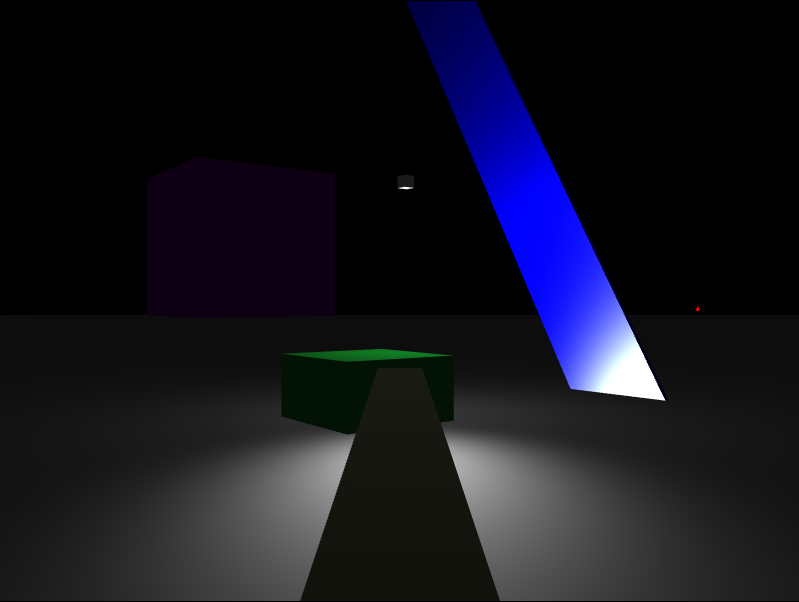
\includegraphics[width=\linewidth]{Cap-Desenvolvimento/gamedoom.png}
  \caption{Jogo implementado utilizando-se a framework}
  \label{des:gamedoom}
\end{figure}

O código desenvolvido pode ser encontrado em \url{https://github.com/Ghust1995/my-cpp-engine/tree/love-like}

